\chapter{Introduction}\label{chap:intro}

This project is devised as a part of the B.Sc. Robot Systems Engineering, 4th term course at the Faculty of Engineering, University of Southern Denmark, Odense spring 2012. The implicit goal is to obtain basic knowledge of embedded systems. This is because embedded systems figure as a significant part of robots as these systems often controls actuators and process sensor inputs for controlling the robot. Therefore it is also demanded for students participating in this course to grasp the basic concepts of classic and modern control theory. Coupling control theory and embedded systems demand understanding of the basics of real time systems, digital systems, embedded systems and control systems. Applying this knowledge in the real world will be as significant as grasping the concepts.

Because the DSMI\footnote{The Engineering Education Model of the University of Southern Denmark} model is used as a framework for this particular education, it is required for the students participating in this course to formulate a strategy for solving an assignment in teams.

\section{Project description}
The purpose of the project work is to construct a control system for the pan/tilt frame shown in figure \ref{fig:pantiltsystem}, so that it is possible to control it with one or more user inputs. For example a joystick, a keyboard, buttons or via commands from a computer. In addition the system should also provide the user with options for feedback of significant system parameters. This is to be prioritized in the project:
\begin{itemize}
  \item A system analysis and modelling of the individual elements of the system.
  \item Analysis and design of the regulation loops in Matlab and Simulink.
  \item Documentation of FPGA design and implementation.
  \item Documentation of the design and implementation of microprocessor program, including choice of operating system.
  \item Test and verification of the system.
\end{itemize}



It is up to the project group to choose the characteristics of the regulator system and the regulator loops.

\begin{figure}[htb]
	\centering
	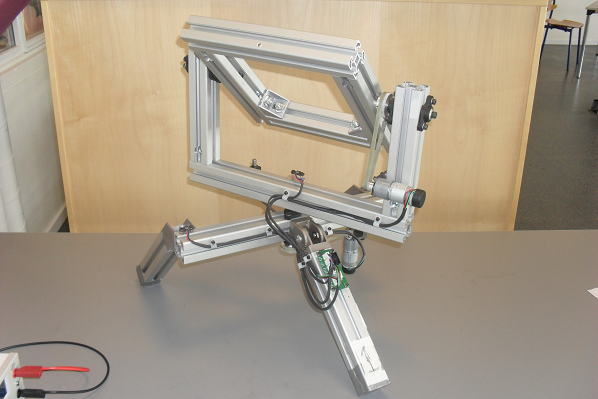
\includegraphics[width=\textwidth]{graphics/pantiltsystem.png} %trim=l b r t
	\caption{The pan/tilt system.}
	\label{fig:pantiltsystem}
\end{figure}

\pagebreak
\section{Requirements}
The following conditions are set for the system:
\begin{itemize}
\item The controller must be implemented on a microprocessor.
\item SPI must be used as the method of communication between the microprocessor and the FPGA.
\item The FPGA must control the PWM signals to the motors.
\item The FPGA must be used to determine the motors positions through use of  their built-in encoders.
\end{itemize}